\documentclass{article}
\usepackage[utf8]{inputenc}
\usepackage{amsmath}
\usepackage{amsthm}
\usepackage[left=1in,right=1in,top=1in,bottom=1in]{geometry}
\usepackage{graphicx}
\usepackage{float}
\usepackage{titling}
\usepackage{algorithm}
\usepackage[noend]{algpseudocode}
\usepackage[numbib,nottoc]{tocbibind}
\usepackage{enumitem}
\setlist[itemize]{topsep=0pt}
\setlist[enumerate]{topsep=0pt}
\setlength\parindent{0pt}
\setlength{\droptitle}{-1.5cm}

\setlength{\abovedisplayskip}{0pt}
\setlength{\belowdisplayskip}{0pt}
\setlength{\abovedisplayshortskip}{0pt}
\setlength{\belowdisplayshortskip}{0pt}

\newcounter{heuristic} \setcounter{heuristic}{0}
\renewcommand{\theheuristic}{\Alph{heuristic}}

\newenvironment{heuristic}[1]%
{
\refstepcounter{heuristic}
\subsection*{Heuristic \theheuristic: #1}
\vspace{-0.2cm}
}%
{}

\makeatletter
\def\BState{\State\hskip-\ALG@thistlm}
\makeatother

\title{Vertex Coloring and Applications}
\date{May 5, 2017}
\author{Shawn Seymour\\ University of Minnesota Morris}

\makeatletter
\def\thm@space@setup{\thm@preskip=8pt
\thm@postskip=0pt}
\makeatother

\newtheorem{prop}{Proposition}
\newtheorem{theorem}{Theorem}

\theoremstyle{definition}
\newtheorem{definition}{Definition}

\begin{document}

\maketitle

\setlength{\parskip}{0.3cm}

\section{Introduction}
Consider the map of the 48 contiguous states in the USA. Suppose we would like to color each state such that no two states that share a boundary have the same color. How many colors would it take to do this? This problem can be modeled as a \emph{graph}. In general, we could represent every state with a \emph{vertex} and draw an \emph{edge} between two states that share a border. A graph, denoted $G = (V, E)$, is a set of vertices $V$ and a set of edges $E$. A \emph{simple graph} is a loopless, undirected graph where no two edges connect the same pair of vertices. For our purpose, assume all graphs are simple graphs. This problem, along with many others, can be solved using vertex coloring.

\begin{figure}[H]
\centering
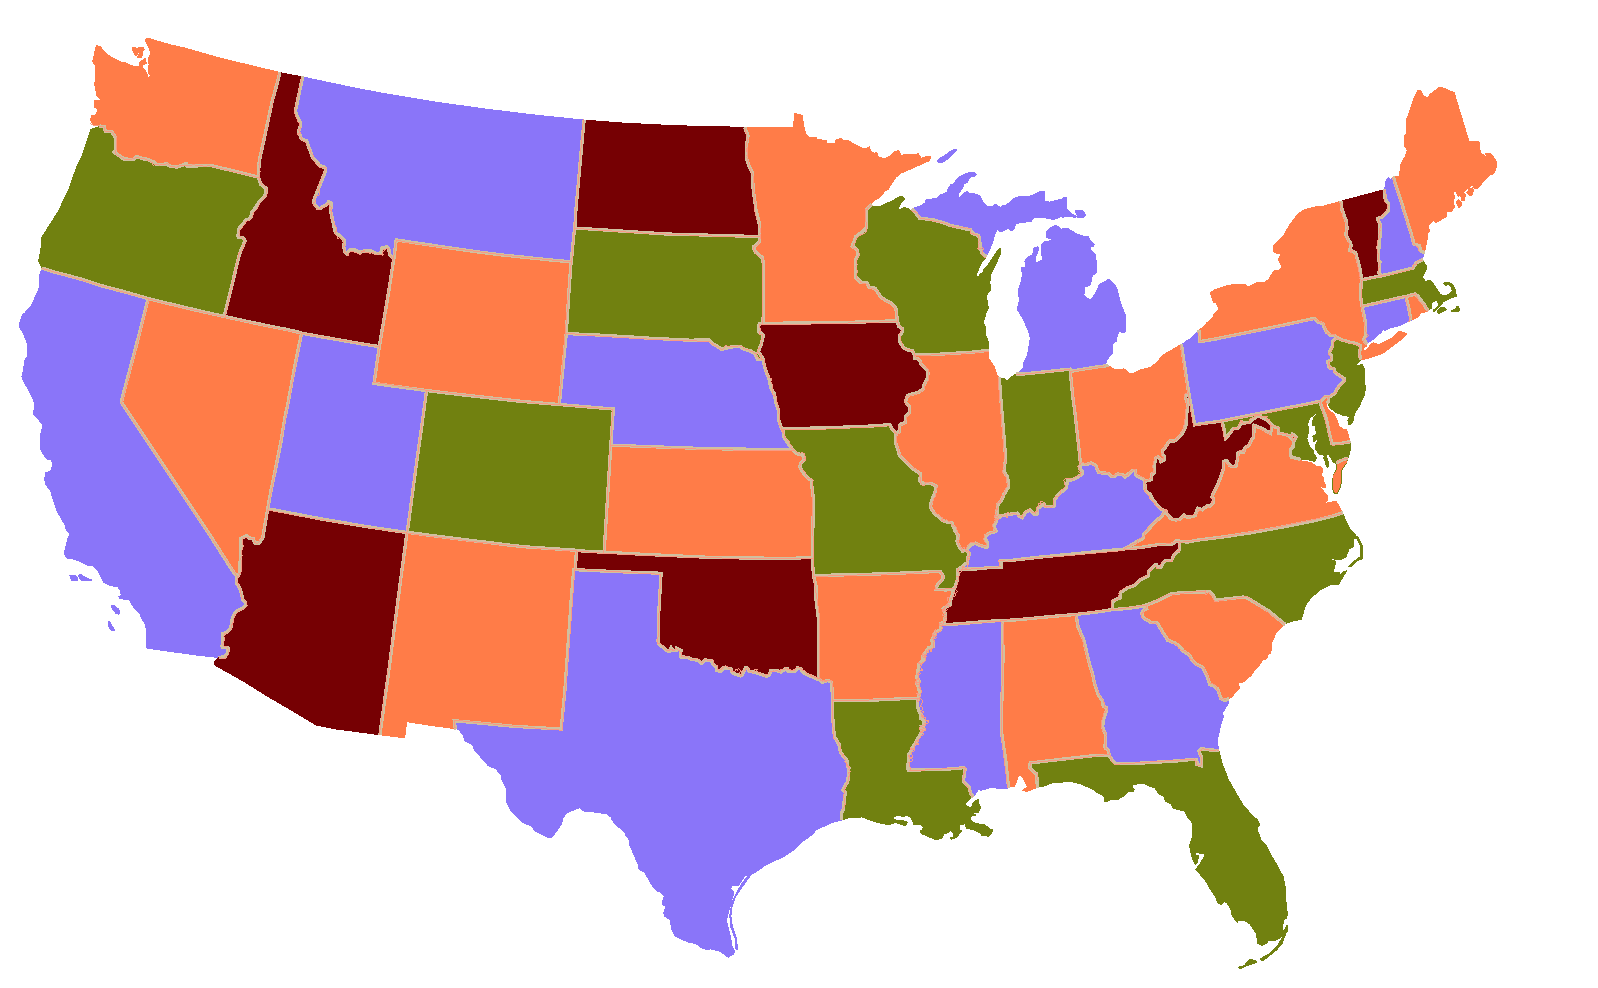
\includegraphics[width=0.7\linewidth]{figures/map-colors.pdf}
\caption{A proper coloring of the USA}\label{fig:map}
\end{figure}

A \emph{vertex coloring} of a graph $G$ is an assignment of colors to each vertex of a graph. A \emph{proper vertex coloring} assigns colors to a graph $G$ such that no two adjacent vertices share the same color. This can be described as a function $f : V \rightarrow S = \{1, 2, \ldots, k\}$ such that $\forall u,w \in V$, if $(u,w) \in E$, then $f(u) \neq f(w)$. Note that this constraint is the same constraint we applied to our map example. This means we could color our map according to our constraint with a proper vertex coloring. For our purpose, assume we mean proper vertex coloring when referring coloring a graph.

The \emph{chromatic number}, denoted $\chi(G)$, is the minimum number of colors needed to have a proper vertex coloring of a graph $G$. The \emph{vertex coloring problem} (VCP), when given a graph $G$, is to find $\chi(G)$. By applying the vertex coloring problem to our map example, we can determine how many colors one would need to color it with regards to our constraint. An example coloring of our map is shown in Figure \ref{fig:map}. The \emph{k-Colorability problem} asks if a graph can be colored with $k$ colors. If a graph can be colored with $k$ colors, it is said to be \emph{k-colorable}.

\section{Computational Complexity}\label{sec:complexity}
Finding an optimal solution to the vertex coloring problem is not easy. As the VCP is an optimization problem with regards to a constraint, we know it will require heavy computation to find an optimal solution. In mathematics and computer science, we classify computationally complex problems based on type of problem they are and based on how many steps it takes to solve the problem with respect to its input size.

\subsection{Classifying the Vertex Coloring Problem}
We call any problem that can be answered with ``yes'' or ``no'' a \emph{decision problem}. To classify the vertex coloring problem, we must first introduce some classes, defined in \cite{moret}:

\begin{itemize}
  \item \textbf{P}: Given a decision problem, we can solve the problem in polynomial time.
  \item \textbf{NP}: Given a decision problem, we can verify if a given solution is correct in polynomial time but cannot solve the problem in polynomial time.
  \item \textbf{NP-hard}: Given any problem, it is at least as hard as NP problems. They do not have to be in NP, however, as they do not need to have solutions verifiable in polynomial time.
  \item \textbf{NP-complete}: Given a decision problem, we can transform it to any other NP problem in polynomial time and still verify a given solution in polynomial time.
\end{itemize}

Take note that these classes are not exclusive: any member of P is also a member of NP. NP-complete problems can be thought of as the problems that are both in NP and NP-hard. Although it may seem like all problems that are NP are also NP-complete, this is not the case. There are a select few problems in NP that are not NP-complete or in P \cite{ladner1975structure}.

\begin{prop}
The vertex coloring problem is an NP-hard problem.
\end{prop}

It is NP-hard to compute the chromatic number of a graph. This can be proven by showing it is at least as hard as a problem in NP. This is typically done by a reduction (a transformation) to or from 3-SAT, which we'll examine later. This is proven in \cite{garey}.

\begin{prop}\label{prop:k-color-np-complete}
The k-Colorability problem, i.e. can a given graph be colored in k-colors, is NP-complete.
\end{prop}

To prove this, we need to reduce a known NP-complete problem to the vertex coloring problem in polynomial time. By reducing a known NP-complete problem to k-Colorability, we can conclude that k-Colorability is NP-complete as all NP-complete problems are reducible to all other NP-complete problems \cite{gareynp}. We will reduce the well-known 3-SAT problem first to the 3-Colorability problem. The 3-Colorability problem asks if a graph can be colored with 3 (or fewer) colors. Obviously, if a graph can be colored with 2 colors it can also be colored with 3.  From here, the reduction from 3-Colorability to k-Colorability follows.

\subsection{Reduction from 3-SAT to 3-Colorability}
Before we prove Proposition \ref{prop:k-color-np-complete}, we must first introduce 3-SAT.  The 3-SAT problem is an NP-complete problem that is a variation of the original NP-complete problem, boolean satisfiability (SAT). The 3-SAT problem is defined and proven to be NP-complete in \cite{gareynp}. 3-SAT consists of a conjunction of a number of clauses. A clause is a disjunction of a given number of propositions or their negations. We will assume all of our satisfiability problems are in conjunctive normal form (CNF). 3-SAT asks whether the variables can be assigned \emph{true} or \emph{false} in such a way that the whole expression evaluates to \emph{true}. We define SAT and 3-SAT in Definition \ref{def:sat}.

\begin{definition}\label{def:sat}
SAT is a conjunction of $m$ clauses, i.e. $C_1 \wedge C_2 \wedge \dots \wedge C_m$. Each clause is a disjunction of at most $n$ literals, i.e. $L_1 \vee L_2 \vee \dots \vee L_n$. Each literal can be a variable or negative of a variable, i.e. $x_1, \neg x_1, x_2, \neg x_2, \dots , x_k, \neg x_k$ where $k$ is the number of distinct literals. Each literal has a value of $true$ or $false$. 3-SAT is where each clause has exactly 3 literals \((n = 3)\).
\end{definition}

To show a reduction from 3-SAT to 3-Colorability, we need to:

\begin{enumerate}
\item Given an instance of 3-SAT, construct an instance of 3-Colorability
\item Show that if the resulting graph is 3-colorable, then the given 3-SAT problem is satisfied
\end{enumerate}

To show this reduction, we'll create an example 3-SAT problem and reduce it to 3-Colorability. This reduction will create a graph \(G = (V, E)\) having \((2n + 3m + 1)\) vertices and \((3n+6m)\) edges \cite{moret}. The process for creating the graph, described below, was taken from the proof given in \cite{sharma}.

Let's introduce the following 3-SAT expression $E$:
%
\begin{align*}
E = \left( x_1 \vee \neg x_2 \vee \neg x_3 \right) \wedge \left( \neg x_1 \vee x_2 \vee x_3 \right) \wedge \left( x_1 \vee x_2 \vee x_3 \right)
\end{align*}
%
To create the graph of this 3-SAT problem, we:
\begin{enumerate}
\item Create a \emph{triangle} for each variable, i.e. \(x_i\). Each has a common vertex \(B\), called the base vertex. This base vertex will be colored a color, say \(p_1\), so that the other two vertices correspond to the variable and it's negation.
\item Create a \emph{triangle} for each clause in the formula.
\item Connect each vertex of a clause triangle to the corresponding literal vertex.
\end{enumerate}

Following the above steps, we generate graph $G$, shown in Figure \ref{fig:3sat1}, from our 3-SAT expression $E$.

\begin{figure}[H]
\centering
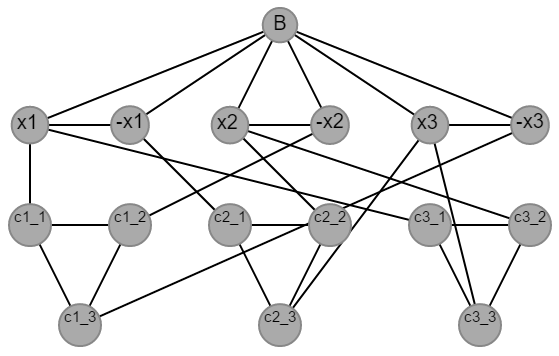
\includegraphics[scale=0.6]{images/3sat-1.png}
\caption{\(E\) represented as a graph \(G\)}\label{fig:3sat1}
\end{figure}

If we can properly color graph \(G\) with 3 colors, then the original 3-SAT is satisfiable and the truth values of the variables are denoted by the color they received. This graph is \emph{3-colorable} and the coloring is shown in Figure \ref{fig:3sat2}.

\begin{figure}[H]
\centering
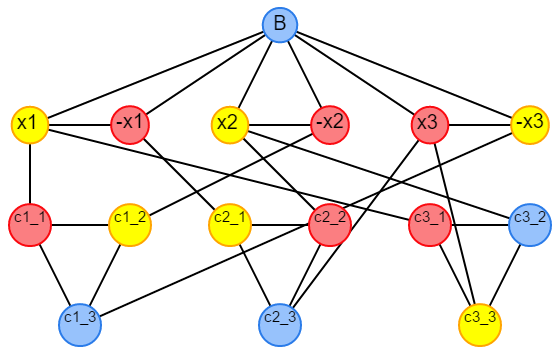
\includegraphics[scale=0.6]{images/3sat-2.png}
\caption{A possible 3-coloring of \(G\)}\label{fig:3sat2}
\end{figure}

As we see above, \emph{blue} is used for the base vertex and as part of some of the clause triangles. If we let \emph{yellow} denote \emph{true} and \emph{red} denote \emph{false}, we can see that our original 3-SAT is satisfied:
%
\begin{align*}
E &= \left( T \vee \neg T \vee \neg F \right) \wedge \left( \neg T \vee T \vee F \right) \wedge \left(T \vee T \vee F \right) \\
&= \left( T \vee F \vee T \right) \wedge \left( F \vee T \vee F \right) \wedge \left(T \vee T \vee F \right) \\
&= T \wedge T \wedge T \\
&= True
\end{align*}
%
This shows an example of the reduction from 3-SAT to 3-Colorability. If \(G\) was unable to be colored with 3 colors, then we would know that \(E\) is unable to be satisfied. From here, we can reduce 3-Colorability to 4-Colorability, and then generalize that reduction and reduce 4-Colorability to k-Colorability. The proof and illustration of this can be found in \cite{sharma}.

\section{Heuristics}
As we have seen in section \ref{sec:complexity}, solving the vertex coloring problem requires heavy computation. This gives us incentive to use approximation algorithms, called heuristics, to find good, but not necessarily optimal, vertex colorings. We decided to analyze and compare a few of the popular heuristics for solving the VCP. The input for all heuristics we define is a simple graph, $G = (V, E)$.

\heuristic{Greedy}\label{heuristic-greedy}

Heuristic \ref{heuristic-greedy} is a simple greedy algorithm. It is defined in Algorithm \ref{alg:greedy}.

\begin{algorithm}
\caption{Greedy algorithm}\label{alg:greedy}
\begin{algorithmic}[1]
\State Label each vertex in $V$, i.e. $v_1, v_2, \dots, v_n$
\For{each $v \in V$}
\State Assign a color $p_i$ to $v_i$ using the smallest available $p_i$
\EndFor
\end{algorithmic}
\end{algorithm}

\heuristic{Welsh-Powell}\label{heuristic-welsh}

Heuristic \ref{heuristic-welsh} is the greedy algorithm with degree sequencing. Before applying the greedy algorithm, it orders the vertices according to the decreasing value of their degree. This is also known as the Welsh-Powell algorithm, which is given in \cite{welsh}. It is defined in Algorithm \ref{alg:welsh}.

\begin{algorithm}
\caption{Welsh-Powell algorithm}\label{alg:welsh}
\begin{algorithmic}[1]
\State Label each vertex in $V$, i.e. $v_1, v_2, \dots, v_n$, such that $d_G(v_1) \geq d_G(v_2) \geq \dots \geq d_G(v_n)$
\ForAll{$v \in V$}
\State Assign a color $p_i$ to $v_i$ using the smallest available $p_i$
\EndFor
\end{algorithmic}
\end{algorithm}

\heuristic{DSATUR}\label{heuristic-dsatur}

Heuristic \ref{heuristic-dsatur} is very similar to heuristic \ref{heuristic-welsh}, but colors a graoh based on the \emph{saturation} degree of vertices, which is defined in Definition \ref{def:sat} \cite{spinrad}. The original DSATUR algorithm was proposed by \cite{brelaz}. It is defined in Algorithm \ref{alg:dsatur}.

\begin{definition}[Saturation degree]\label{def:sat}
The saturation degree of a vertex is the number of different colors used for vertices adjacency to it.
\end{definition}

\begin{algorithm}
\caption{DSATUR algorithm}\label{alg:dsatur}
\begin{algorithmic}[1]
\State Find the vertex $\in V$ with maximum degree and color it with color $p_1$
\While{There are uncolored vertices}
\State Choose an uncolored vertex with maximum saturation degree
\State If there is a tie, choose the vertex with maximum degree
\State Color the vertex with the least possible number
\EndWhile
\end{algorithmic}
\end{algorithm}

\heuristic{Maximal Independent Set}\label{heuristic-mis}

Heuristic \ref{heuristic-mis} colors a graph by finding maximal independent sets of \(G\). A maximal independent set (MIS) is defined in Definition \ref{def:mis}. This is quite different than our other heuristics as it does not depend on degree. Ideally, we would want to find a maximum independent set, not just a maximal independent set.

Finding a maximum independent set is NP-hard \cite{karp1972reducibility}, however, meaning we're including a different NP-hard in an already NP-hard problem. We chose to forgo this in favor of just finding a maximal independent set. We define the heuristic in Algorithm \ref{alg:mis}.

\begin{definition}[Maximal independent set]\label{def:mis}
An independent set is a subset $S$ of vertices in a graph such that no two vertices in the set are adjacent. $S$ is said to be maximal if no vertex outside the set can be added while still being an independent set.
\end{definition}

\begin{algorithm}
\caption{Maximal independent set algorithm}\label{alg:mis}
\begin{algorithmic}[1]
\State $p \leftarrow 1$
\While{$G$ is non-empty}
\State Find a maximal independent set of $G$, i.e. $S_i$
\State Color all vertices in $S_i$ with color $p$
\State Let $G \leftarrow G[V \setminus S_i ] $
\State $p \leftarrow p + 1$
\EndWhile
\end{algorithmic}
\end{algorithm}

\section{Initial Findings}
Before comparing the heuristics, we first wanted to analyze the heuristics individually and look at the solutions they produce.

\begin{prop}
Heuristic \ref{heuristic-greedy} and Heuristic \ref{heuristic-welsh} produce a feasible, proper coloring of input graph \(G = (V, E)\).
\end{prop}

Let \(G = (V, E)\) be a simple graph. Assume that two vertices, say \(v_1, v_2 \in V\), are connected by an edge \(e_1 \in E\). Assume that \(v_1, v_2\) are colored the same color, say \(p_1\). We know that in both heuristics, we assign the smallest color \(p_i\) that is not being used by any of the neighboring vertices connected by an edge \(e_i\). WLOG, the heuristic would color \(v_1\) color \(p_1\). The next iteration, while vertex \(v_2\) is selected, the heuristic would see color \(p_1\) is assigned to a neighboring vertex \((v_1)\), and assign the next available color \(p_2\). Thus, we've reached a contradiction.

\begin{prop}
Heuristic \ref{heuristic-dsatur} produces a feasible, proper coloring of input graph \(G = (V, E)\).
\end{prop}

Let \(G = (V, E)\) be a simple graph. We color the vertex with the maximum degree color 1. If there are no uncolored vertices, we have properly colored $G$. If there are, then we find an uncolored vertex $v$ with maximum saturation degree. We then color $v$ with the smallest available color. This means we look at the set of all adjacent vertices to $v$ and find the smallest unused color in this set. This means we will never color an adjacent vertex with the same color, and thus, will always result in a proper coloring.

\begin{prop}
Heuristic \ref{heuristic-mis} produces a feasible, proper coloring of input graph \(G = (V, E)\).
\end{prop}

Let \(G = (V, E)\) be a simple graph. Let $p$, the current color, be 1. By definition \ref{def:mis}, we know that no two vertices in a maximal independent set are adjacent. Thus, when we color the vertices in the MIS with the smallest color \(p_1\) for the first iteration, we know that it is properly colored. We then remove the found maximal independent set and increment $p$ to 2. If $G$ is now empty, then $G$ is properly colored. If $G$ is not empty, then we repeat the process except we use color 2. Because we are always incrementing the color for each iteration, we know the MIS found will always be properly colored with a different color than the past MIS.

Now that we know our heuristics produce feasible, proper colorings of a graph, how do we know they do not produce optimal solutions? We show they do not using counterexamples. 


\newpage

\bibliographystyle{abbrv}
\bibliography{references}


\end{document}
